\section{Introduction}

\begin{example}
\label{example:loop}
We use an example through the paper to illustrate 
the concepts.
Consider the network depicted in figure \ref{fig:loop}.
In this network, we have four switches and solid arrows show 
the initial routes.
Assume that two concurrent updates $p,q$ will happen in the network.
The update $p$ replaces the route $cd$ with $cbd$ and 
$q$ replaces the route $abc$ with $ac$.
Assume that we require to ensure that no loop appears in the network at 
any given time.
If $q$ happens before $p$ then we have loop in network between the $b$ 
and $c$.
But if $q$ happens after $p$ no loop appears in the network and we reach
the desired state without violating the loop-freedom property.
In the following, we explain how we can use the causal model to show that the 
lack of ordering between $p$ and $q$ is an actual cause of 
the loop-freedom violation.
\end{example}

\begin{figure}
    \centering
    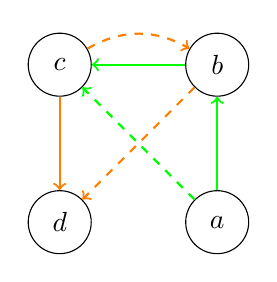
\begin{tikzpicture}[node distance={20mm},main/.style = {draw, circle,minimum size=8mm}]
        \node[main] (a)  {$a$};
        \node[main] (b) [above of=a]  {$b$};
        \node[main] (c) [left of=b] {$c$};
        \node[main] (d)  [below of=c] {$d$};
        \draw [->,green,thick] (a) -- (b);
        \draw [->,green,thick] (b) -- (c);
        \draw [->,orange,thick] (c) -- (d);
        \draw [->,green,thick,dashed] (a) -- (c);
        \draw [->,orange,thick,dashed] (c) edge[bend left] (b);
        \draw [->,orange,thick,dashed] (b) -- (d);
    \end{tikzpicture}
    \caption{Loop-freedom example}
    \label{fig:loop}
\end{figure}